\chapter{Control automático desde cero}

\begin{enpocas}
Qué es controlar, la diferencia entre lazo abierto y lazo cerrado, el error, los controladores P, PD
y PID, cómo se lee una respuesta y por qué un dron necesita control en cascada.
\end{enpocas}

\section{¿Qué es controlar?}

Controlar es conseguir que algo se comporte como queremos aunque haya perturbaciones. Queremos que el
dron esté a 30~m de altura; el viento lo empuja hacia abajo; el controlador acelera los motores para
compensar. Al ``algo'' que se controla se le llama \textbf{planta} (aquí, el dron); a lo que queremos,
\textbf{referencia} o \textbf{consigna}; a lo que nos estorba, \textbf{perturbación}.

\section{Lazo abierto y lazo cerrado}

\begin{figure}[H]
\centering
\begin{tikzpicture}[blq/.style={draw,rounded corners,fill=#1,minimum width=2.4cm,minimum height=0.9cm,align=center,font=\small},blq/.default=white,
  fl/.style={-{Stealth[length=2.2mm]},thick}, sum/.style={draw,circle,inner sep=1.5pt}]
  \node at (-1.4,0.9) {\textbf{Lazo abierto}};
  \node (r1) at (-1.2,0) {referencia};
  \node[blq=blue!10] (c1) at (2,0) {controlador};
  \node[blq=orange!15] (p1) at (5.5,0) {planta\\(dron)};
  \node (y1) at (8.6,0) {salida};
  \draw[fl] (r1) -- (c1); \draw[fl] (c1) -- node[above,font=\scriptsize]{acción} (p1); \draw[fl] (p1) -- (y1);
  \node (d1) at (5.5,1.3) {perturbación}; \draw[fl] (d1) -- (p1);

  \node at (-1.4,-1.7) {\textbf{Lazo cerrado}};
  \node (r2) at (-1.2,-2.6) {referencia};
  \node[sum] (s) at (0.5,-2.6) {$-$};
  \node[blq=blue!10] (c2) at (2.6,-2.6) {controlador};
  \node[blq=orange!15] (p2) at (5.9,-2.6) {planta\\(dron)};
  \node (y2) at (9,-2.6) {salida};
  \node[blq=green!12] (sen) at (5.9,-4.1) {sensor};
  \draw[fl] (r2) -- (s); \draw[fl] (s) -- node[above,font=\scriptsize]{error} (c2); \draw[fl] (c2) -- node[above,font=\scriptsize]{acción} (p2);
  \draw[fl] (p2) -- (y2); \draw[fl] (8.1,-2.6) |- (sen); \draw[fl] (sen) -| (s);
  \node (d2) at (5.9,-1.3) {perturbación}; \draw[fl] (d2) -- (p2);
\end{tikzpicture}
\caption{En lazo abierto se actúa ``a ciegas''. En lazo cerrado se mide el resultado, se compara con
lo que se quiere y se corrige: eso es la \emph{retroalimentación}.}
\end{figure}

\begin{ejemplo}
Una tostadora es lazo abierto: tuesta un tiempo fijo, aunque el pan se queme. Ajustar la temperatura
de la regadera es lazo cerrado: sientes el agua (sensor), la comparas con la que quieres (error) y
mueves la llave (acción). Si alguien abre otra llave en la casa (perturbación), lo notas y corriges.
\end{ejemplo}

Un dron sin lazo cerrado no se puede volar: cualquier ráfaga o diferencia entre motores lo voltea
en un segundo. El \textbf{error} es la diferencia entre lo que queremos y lo que hay,
$e = \text{referencia} - \text{medición}$, y todo controlador hace algo con él.

\section{El controlador proporcional (P)}

La idea más simple: actuar en proporción al error. Si estoy 2~m abajo, empujo el doble que si estoy
1~m abajo:
\begin{equation}
u = K_p\, e .
\end{equation}
$K_p$ es la \textbf{ganancia proporcional}. El problema con un dron: el control P actúa sobre la
\emph{aceleración}, y un objeto que se acelera hacia el objetivo llega con velocidad, se pasa,
regresa, se vuelve a pasar... oscila para siempre (curva gris de la figura~\ref{fig:pid}).

\section{El término derivativo (D): frenar a tiempo}

Hay que frenar antes de llegar. El término derivativo actúa sobre la \emph{velocidad} del error: si
me acerco rápido, freno.
\begin{equation}
u = K_p\, e + K_d\, \dot e .
\end{equation}
Es como un amortiguador. Con poco $K_d$ oscila; con mucho, llega muy lento; hay un punto intermedio
(figura~\ref{fig:pid}, derecha).

\section{El término integral (I): no rendirse}

Si un viento constante empuja hacia abajo, el PD llega a un equilibrio un poco por debajo del
objetivo: con ese pequeño error ya compensa el viento. El término integral \emph{acumula} el error en
el tiempo: mientras haya error, sigue creciendo hasta eliminarlo.
\begin{equation}
u = K_p\, e + K_d\, \dot e + K_i\!\int e\,dt .
\end{equation}

\begin{figure}[H]
\centering
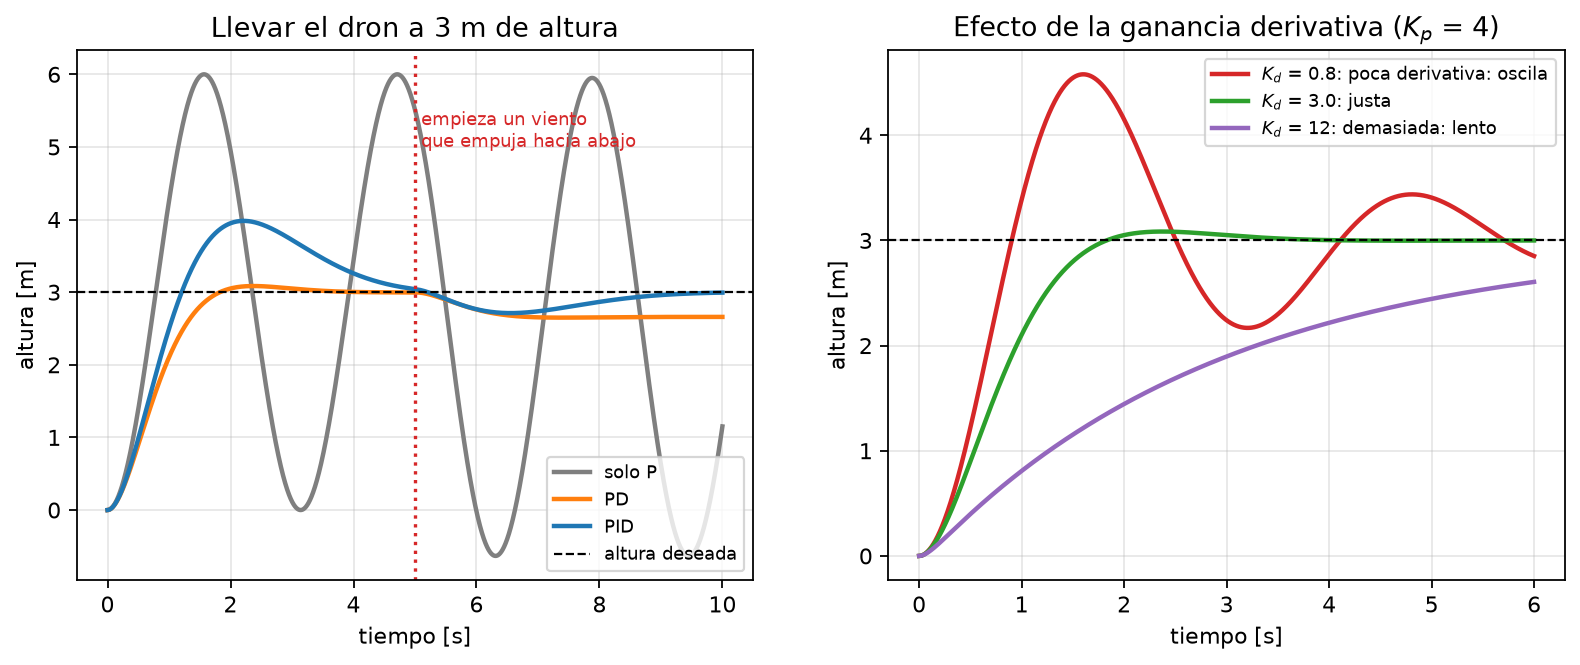
\includegraphics[width=\textwidth]{c_pid.png}
\caption{Simulación de la altura de una masa de 2.2~kg (como el Tarot). Izquierda: solo P oscila; PD
llega pero el viento (desde $t=5$~s) le deja un error; PID lo corrige. Derecha: efecto de $K_d$.}
\label{fig:pid}
\end{figure}

\begin{recuerda}
\textbf{P} empuja hacia el objetivo, \textbf{D} frena para no pasarse, \textbf{I} corrige lo que
queda. El PID es, de lejos, el controlador más usado en el mundo, incluidos los drones comerciales.
\end{recuerda}

\section{Cómo se lee una respuesta}

Para comparar controladores se les pide un cambio brusco de referencia (un \textbf{escalón}) y se
mide:

\begin{figure}[H]
\centering
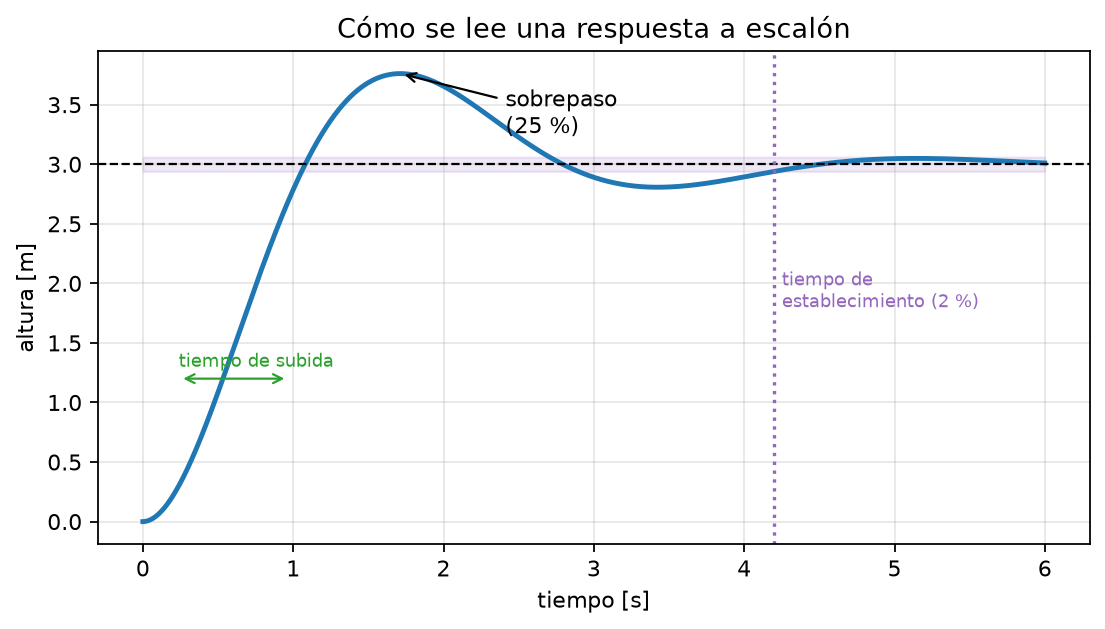
\includegraphics[width=0.8\textwidth]{c_respuesta.png}
\caption{Medidas típicas de una respuesta a escalón.}
\end{figure}

\begin{description}
  \item[Sobrepaso:] cuánto se pasa del objetivo.
  \item[Tiempo de subida:] cuánto tarda en ir del 10~\% al 90~\% del cambio.
  \item[Tiempo de establecimiento:] a partir de cuándo se queda cerca del objetivo (por ejemplo, a
        menos del 2~\%).
  \item[Error en estado estacionario:] lo que queda de error cuando todo se calma.
\end{description}
En este proyecto se usa sobre todo el \textbf{error RMS} (raíz del promedio de los errores al cuadrado)
durante una órbita con viento: un solo número que resume qué tan bien sigue el dron su trayectoria.

\section{Control en cascada: así se controla un dron}

El dron no puede ``moverse a la derecha'' directamente: tiene que inclinarse. Por eso hay dos lazos,
uno dentro del otro:

\begin{figure}[H]
\centering
\begin{tikzpicture}[blq/.style={draw,rounded corners,fill=#1,minimum width=2.6cm,minimum height=1cm,align=center,font=\small},blq/.default=white,
  fl/.style={-{Stealth[length=2.2mm]},thick}]
  \node (ref) at (-0.6,0) {\small posición deseada};
  \node[blq=blue!10] (pos) at (2.6,0) {lazo de posición\\(lento: PD o STA)};
  \node[blq=red!10] (act) at (6.4,0) {lazo de actitud\\(rápido: PD en SO(3))};
  \node[blq=black!5] (mix) at (10,0) {mezclador};
  \node[blq=orange!15] (dron) at (10,-2.2) {dron};
  \draw[fl] (ref) -- (pos);
  \draw[fl] (pos) -- node[above,font=\scriptsize,align=center]{empuje e\\inclinación} (act);
  \draw[fl] (act) -- node[above,font=\scriptsize]{pares} (mix);
  \draw[fl] (mix) -- node[right,font=\scriptsize]{4 velocidades} (dron);
  \draw[fl] (dron.west) -- ++(-3,0) -| node[pos=0.75,right,font=\scriptsize]{orientación} (act.south);
  \draw[fl] (dron.west) -- ++(-6.8,0) -| node[pos=0.75,right,font=\scriptsize]{posición} (pos.south);
\end{tikzpicture}
\caption{Control en cascada del cuadrirrotor.}
\label{fig:cascada}
\end{figure}

\begin{enumerate}
  \item El \textbf{lazo de posición} compara dónde está el dron con dónde debe estar y calcula qué
        fuerza total necesita: cuánto empuje y hacia dónde apuntarlo.
  \item Apuntar el empuje significa inclinar el dron: el \textbf{lazo de actitud} calcula los pares
        para alcanzar esa inclinación. Es mucho más rápido que el de posición.
  \item El \textbf{mezclador} convierte empuje y pares en la velocidad de cada motor.
\end{enumerate}
En este proyecto, el lazo interno es siempre el mismo y lo que se cambia es el externo: el PD
(línea base) o el super-twisting adaptativo, que es el tema del próximo capítulo.

\begin{ejercicio}
Compara el PD con el STA en la órbita con viento:
\begin{lstlisting}[style=bash]
ros2 launch cuadrirotor_sim simulacion.launch.py vehiculo:=tarot650 mundo:=bosque controlador:=pd mision:=orbita viento:=true csv:=$HOME/pd.csv
ros2 launch cuadrirotor_sim simulacion.launch.py vehiculo:=tarot650 mundo:=bosque controlador:=sta mision:=orbita viento:=true csv:=$HOME/sta.csv
python3 ~/ros2_ws/src/cuadrirotor_sim/scripts/metricas.py ~/pd.csv ~/sta.csv
\end{lstlisting}
\end{ejercicio}
